%=============================================================================
% FIT (Frontiers of Information Technology) — IEEE two-column conference format
%
% FIT requirements confirmed from https://fit.edu.pk/submission-guidelines.aspx
%   - two-column IEEE conference format
%   - PDF, submitted via EasyChair
%   - must not be under consideration elsewhere
%
% PAGE BUDGET: not a constraint per the author — write what the work needs.
% Confirm the venue's actual limit before submitting; if over-length pages carry
% a fee, that is a submission-time decision, not a writing-time one.
%
% Build:  pdflatex main && bibtex main && pdflatex main && pdflatex main
% Check the page count EVERY build. The count includes references.
%=============================================================================
\documentclass[conference]{IEEEtran}
\IEEEoverridecommandlockouts

\usepackage{cite}
\usepackage{amsmath,amssymb}
\usepackage{algorithmic}
\usepackage{graphicx}
\usepackage{textcomp}
\usepackage{xcolor}
\usepackage{booktabs}
\usepackage{url}

% Draft-only marker. DELETE this macro and every use of it before submitting.
\newcommand{\TODO}[1]{\textcolor{red}{\textbf{[TODO: #1]}}}

\begin{document}

\title{Grounded and Auditable: Tool-Augmented Retrieval-Generation
with Selective Abstention for Legal Question Answering in
Low-Resource, Code-Switched Jurisdictions}

% IEEE author block. FIT is not double-blind (confirm on the CFP before
\author{\IEEEauthorblockN{Muhammad Usama$^{1}$ and Muhammad Amir Zarmaan Ullah Khan$^{2}$}
\IEEEauthorblockA{\textit{$^{1,2}$Department of Computer Science, COMSATS University Islamabad, Pakistan}\\
Email: \href{mailto:muhammadusamahoyrr@gmail.com}{\underline{muhammadusamahoyrr@gmail.com}}, \href{mailto:kzari898@gmail.com}{\underline{kzari898@gmail.com}}}}

\maketitle

%-----------------------------------------------------------------------------
\begin{abstract}
Retrieval-augmented legal question answering is evaluated almost entirely on
answer quality, leaving two properties that matter more in practice unmeasured:
whether a system knows when \emph{not} to answer, and whether an answer can
later be audited. We present a governance architecture for Pakistani law that
treats both as first-class --- hybrid retrieval over a bilingual statute corpus,
deterministic statutory engines admitted as evidence by the grounding verifier,
Roman-Urdu normalisation, and a single enforced output path that records every
turn --- and report what measuring those properties revealed. Decomposing our
own confidence score gives the principal finding: its highest-weighted component
was \emph{anti-correlated} with answerability, scoring questions the corpus
cannot answer above those it can by $0.343$, a defect that worsened as the
corpus grew and that the aggregate concealed. Correcting it restores the
ordering, yet the answerable and unanswerable distributions still overlap, so no
threshold separates them; we argue abstention here is not a question of degree
in confidence but of the kind of fact requested, and decide it from the query
before evidence is weighed. We further replace a hand-set action-cost vector
with an expected-loss rule over an explicit harm matrix, under which the
operating threshold is the harm ratio by derivation --- revealing that our
deployed threshold had implicitly assumed a missed answer to be four times worse
than a misstatement of law. Our second finding concerns how such systems are
evaluated. Fine-tuning the retriever on domain data yields $+26.5$ Hit@1 when
tested on questions from its own training distribution and $+2.4$ when the
question style changes; a second model, trained independently on a tenth as much
data from a different source, shows the same collapse in the opposite direction.
Sorting every retrieval intervention we measured by whether its gain survived a
change of question style produces a clean split: those encoding legal or
document structure transferred, those learning question phrasing did not,
including a general-purpose cross-encoder that moved the correct statute from
rank~3 to rank~10 where a deterministic statutory-scope rule placed it first in
under a millisecond. Three separate contaminations each inflated a headline number until it
was checked, and each time the flattering version was the wrong one.
\end{abstract}

\begin{IEEEkeywords}
legal informatics, retrieval-augmented generation, selective prediction,
abstention, neuro-symbolic systems, low-resource NLP, code-switching, Urdu
\end{IEEEkeywords}

%-----------------------------------------------------------------------------
\section{Introduction}
Access to legal information is unevenly distributed. A litigant who cannot
afford counsel is often unable to establish even the threshold facts of their
own position: which statute governs, which forum has jurisdiction, what a
filing will cost, or whether a limitation period has already expired.
\TODO{Insert one cited statistic on the lawyer-to-population ratio or case
backlog in Pakistan. Do not write a number you have not sourced.}

Large language models with retrieval augmentation~\cite{lewis2020rag} appear
well suited to closing part of that gap, and legal question answering is now an
active application area~\cite{chalkidis2020legalbert,guha2023legalbench}.
Existing systems, however, are built predominantly for English and for
common-law or European jurisdictions. Transferring them to Pakistan is not a
matter of swapping the corpus. Queries arrive in English, in Urdu script, and
most commonly in Roman Urdu, the transliterated register used in everyday
digital communication; the applicable law combines codified statute with
Islamic personal law and varies by province; and users routinely import Indian
statutory terminology, asking about the Indian Penal Code when the Pakistan
Penal Code governs. Each of these is a retrieval problem before it is a
generation problem.

A second gap is less specific to jurisdiction and, we argue, more consequential.
Legal question-answering systems are evaluated almost entirely on answer
quality, leaving two properties that matter more in practice unmeasured.
\emph{Abstention}: a confidently wrong answer about bail eligibility or a
limitation period can cause material harm, so a system that declines when its
evidence is weak is more useful than one that always responds.
\emph{Auditability}: an answer that cannot be traced to the evidence and
decisions that produced it cannot be contested, corrected, or defended --- which
is precisely what a regulated domain requires. Neither is captured by
answer-quality metrics, and neither is achievable as an afterthought.

This paper describes a legal question-answering system for Pakistani law built
around both. We do not claim a new retrieval or generation model; the components
are largely standard, and deliberately so. The contribution is a
\emph{governance architecture} --- the arrangement that determines which
evidence a verifier will accept, what the system does when the evidence is
weak, which paths may produce output, and what record survives the turn --- and
a set of measurements showing that this arrangement is where the interesting
failures live. Every substantive defect we report was invisible to answer
quality and visible only to the governance layer. Our contributions are:

\begin{itemize}
\item \textbf{Verifier-aware symbolic evidence.} Deterministic statutory
engines --- court fees, bail eligibility, limitation, inheritance shares under
Islamic law --- are treated as first-class evidence by the grounding verifier,
so that a correct computed answer is not mislabelled as ungrounded merely
because no retrieved provision restates it (Section~\ref{sec:tools}).
\item \textbf{An abstention policy derived rather than tuned.} A single
arbitration layer selects among answering, requesting clarification, and
refusing over heterogeneous evidence by minimising expected loss under an
explicit harm matrix, in which an unnecessary refusal is itself a cost. The
operating threshold is the harm ratio by derivation, which makes the assumption
a system encodes about relative harm legible and testable rather than implicit
in a tuned constant (Section~\ref{sec:abstain}).
\item \textbf{Code-switched retrieval} for a low-resource jurisdiction, with
Roman-Urdu normalisation and cross-jurisdictional alias resolution
(Section~\ref{sec:retrieval}).
\item \textbf{Per-turn provenance} linking every emitted answer to its evidence,
its arbitration verdict, and the model that served it, together with an
evaluation protocol that constructs an abstention-aware test set by labelling
recorded traffic (Sections~\ref{sec:prov} and \ref{sec:eval}).
\end{itemize}

\section{Related Work}
\textbf{Legal NLP and retrieval-augmented generation.}
Domain-adapted encoders such as LEGAL-BERT~\cite{chalkidis2020legalbert}
established that legal text benefits from in-domain pretraining, and
LegalBench~\cite{guha2023legalbench} provides a broad benchmark for legal
reasoning in large language models. Retrieval augmentation~\cite{lewis2020rag}
combined with dense passage retrieval~\cite{karpukhin2020dpr} is now the
standard architecture for grounding generated answers in source documents.
Self-RAG~\cite{asai2024selfrag} adds self-reflection over retrieval quality and
answer support. This line of work overwhelmingly targets English and
common-law or EU material, and evaluates the answers produced rather than the
decision of whether to answer.

\textbf{Selective prediction and calibration.}
Selective classification formalises the option to abstain and the
risk--coverage trade-off it induces~\cite{elyaniv2010selective,
geifman2017selectivenet}. Modern neural networks are systematically
miscalibrated~\cite{guo2017calibration}, motivating post-hoc mapping of scores
into probability space by Platt scaling~\cite{platt1999} or isotonic
regression~\cite{zadrozny2002isotonic}; conformal
prediction~\cite{angelopoulos2021conformal} offers distribution-free coverage
guarantees over the same problem. Language models retain some signal about
their own reliability~\cite{kadavath2022know}, and hallucination remains a
central failure mode of generation systems~\cite{ji2023hallucination}. These
techniques are rarely applied to the routing decision inside a retrieval
pipeline, which is where we place them.

\textbf{Tool-augmented and neuro-symbolic generation.}
Delegating exactly-computable subproblems to deterministic components is
well established, but the interaction between tool output and answer
verification is not. Where a grounding check tests whether claims appear in
retrieved text, computed results are structurally invisible to it. We make the
verifier aware of symbolic evidence rather than treating tools purely as a
generation aid.

\textbf{Low-resource retrieval and adversarial robustness.}
Multilingual dense encoders~\cite{wang2024multilinguale5} make a single index
viable across scripts, and hybrid lexical--dense retrieval with rank
fusion~\cite{robertson2009bm25,cormack2009rrf} remains strong where exact
terminology matters, as it does for statute references. Separately, prompt
injection is a practical threat to any deployed instruction-following
assistant~\cite{perez2022ignore,greshake2023injection}. We report a failure mode
in this class that arises from pipeline structure rather than from classifier
weakness.

\begin{table*}[t]
\caption{Positioning against the closest prior work. The final column states
what each line leaves open for a deployed legal assistant, which is what this
paper addresses. No performance figures are compared across rows: the systems
target different jurisdictions, languages and tasks, and a table of headline
accuracies drawn from different datasets would invite exactly the
cross-study comparison Section~\ref{sec:whyleakage} argues against.}
\label{tab:related}
\centering
\small
\begin{tabular}{@{}p{0.15\textwidth}p{0.20\textwidth}p{0.28\textwidth}p{0.28\textwidth}@{}}
\toprule
Line of work & Representative & Contribution & What it leaves open here \\
\midrule
Domain-adapted legal encoders &
\cite{chalkidis2020legalbert,guha2023legalbench} &
In-domain pretraining and benchmarking for legal text &
English common-law/EU text; no abstention decision, and no evidence that
adaptation transfers across question style \\

Retrieval-augmented generation &
\cite{lewis2020rag,karpukhin2020dpr,asai2024selfrag} &
Grounding generated answers in retrieved passages; self-reflection over
retrieval quality &
Evaluates the answer produced, not the decision of \emph{whether} to answer;
retrieval quality is judged, not the query's answerability \\

Selective prediction and calibration &
\cite{elyaniv2010selective,geifman2017selectivenet,guo2017calibration,angelopoulos2021conformal} &
Formalises abstention, the risk--coverage trade-off, and distribution-free
coverage &
Applied to classifier outputs, rarely to the routing decision inside a
retrieval pipeline; the operating point is tuned rather than derived from harm \\

Low-resource and hybrid retrieval &
\cite{wang2024multilinguale5,robertson2009bm25,cormack2009rrf} &
One index across scripts; lexical--dense fusion where exact terminology matters &
Code-switching is treated as a language-identification problem; no account of
what fusion does to a fine-tuned dense channel \\

Prompt-injection robustness &
\cite{perez2022ignore,greshake2023injection} &
Attack taxonomies and classifier defences &
Assumes the defended component is reached; says nothing about paths that
bypass it, which is the failure we report \\
\bottomrule
\end{tabular}
\end{table*}

Table~\ref{tab:related} positions this work against those lines. To our
knowledge, no existing system combines abstention under an explicit cost
model, symbolic evidence admitted by the grounding verifier, and code-switched
retrieval for a low-resource jurisdiction, nor reports an evaluation that
measures all three.

%-----------------------------------------------------------------------------
\section{Method}
\label{sec:method}

\subsection{Overview}

\begin{figure}[t]
\centering
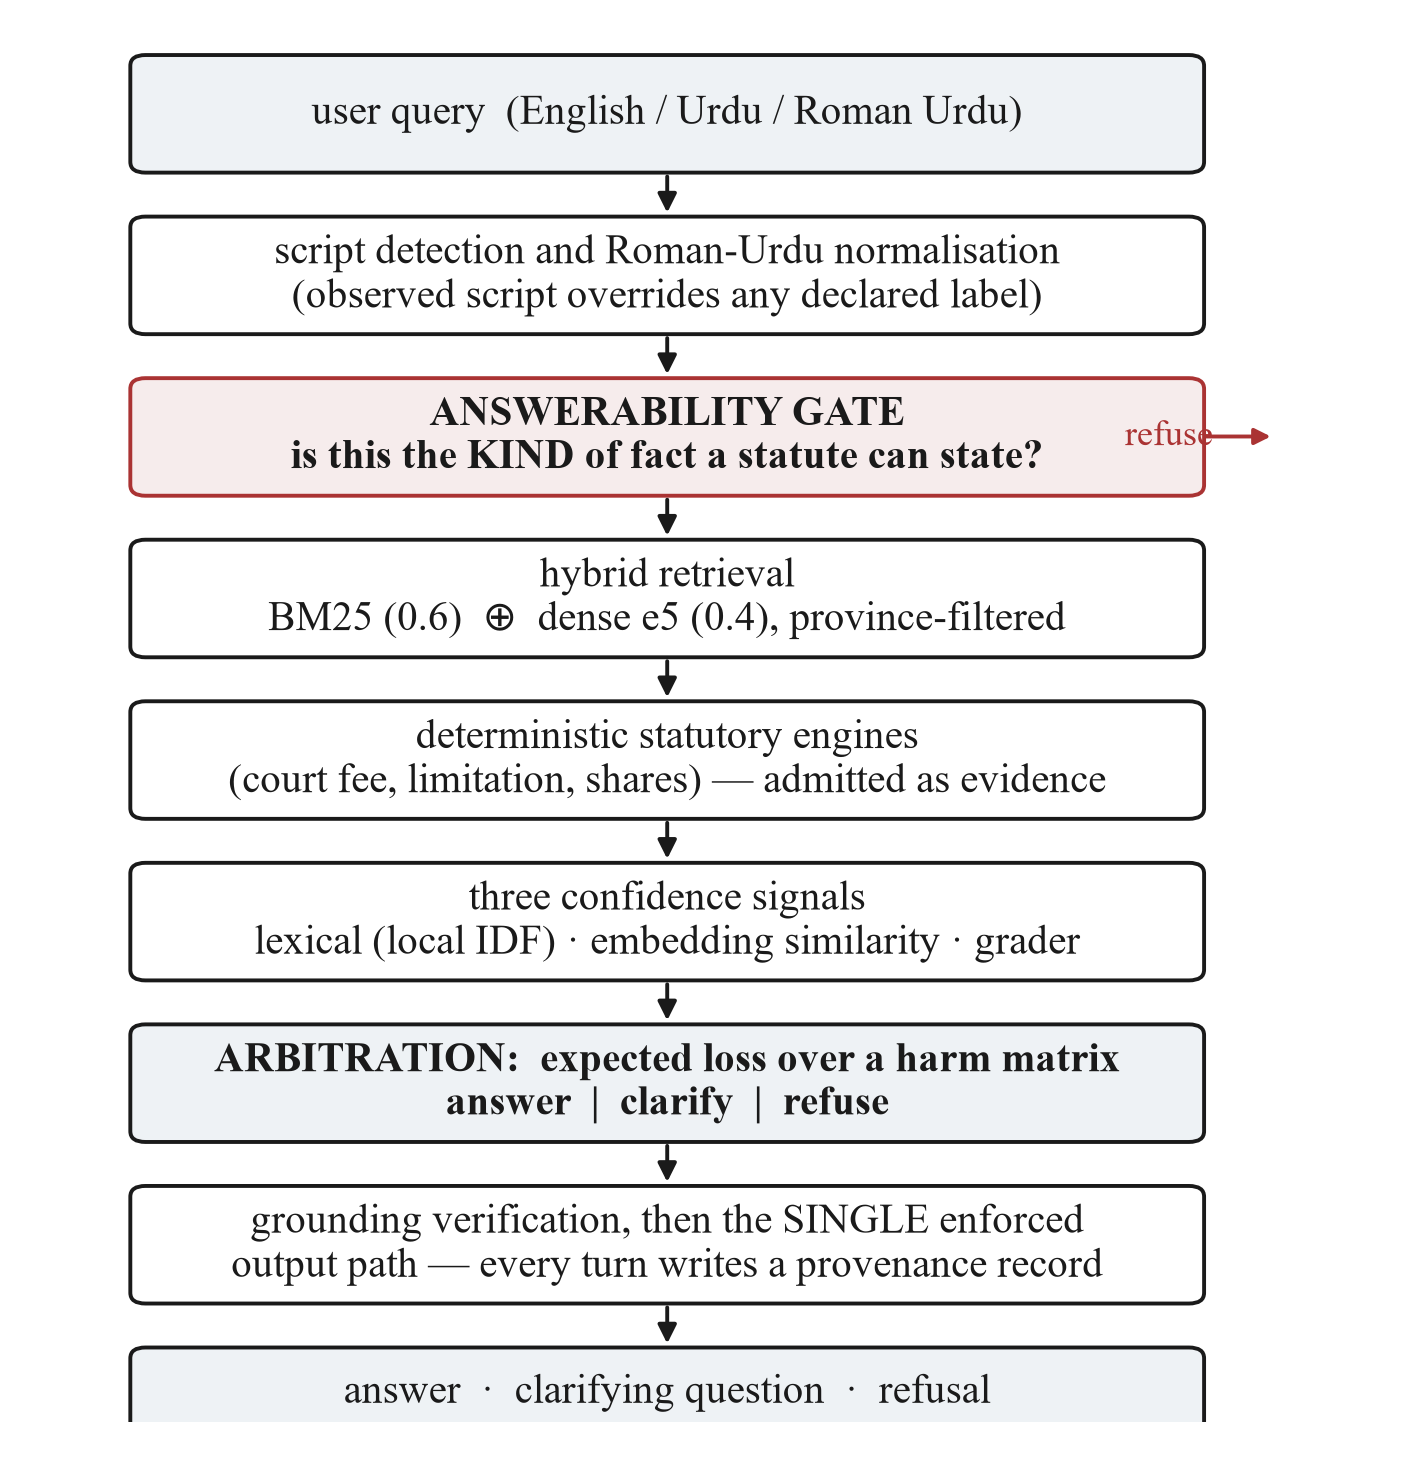
\includegraphics[width=\columnwidth]{figures/fig1_pipeline.png}
\caption{The governance pipeline. Two stages carry the argument of this paper:
the answerability gate, which decides from the \emph{query} whether the corpus
could hold the answer at all, before any evidence is weighed
(Section~\ref{sec:answerability}); and arbitration, whose operating threshold is
derived from a harm ratio rather than tuned (Section~\ref{sec:rho}). Every
branch terminates at one enforced output path, which is what makes the
provenance record of Figure~\ref{fig:prov} complete rather than best-effort.}
\label{fig:pipeline}
\end{figure}

The system is a directed graph of thirteen nodes executed per user turn
(Figure~\ref{fig:pipeline}). A
turn enters an adversarial gatekeeper, is classified and triaged, may be
suspended to ask the user for missing facts, is checked against a semantic
cache, may invoke deterministic statutory engines, retrieves statute and
case-law evidence, has that evidence scored, and only then reaches an
arbitration node that decides whether to answer at all. Generation and a
grounding check follow, and a finaliser sanitises the output. Conversation
state, including the suspended state of a pending clarification, is
checkpointed to a document store so that a turn survives process restarts and
can be resumed by a different worker.

\begin{table}[t]
\caption{Notation used throughout. Symbols are introduced where they first
appear and collected here because several equations share them.}
\label{tab:notation}
\centering
\small
\begin{tabular}{@{}ll@{}}
\toprule
Symbol & Meaning \\
\midrule
$s$ & composite confidence, \eqref{eq:score} \\
$k,\,\hat{e},\,\hat{\ell}$ & lexical, embedding and grader signals \\
$T,\,C$ & content terms of one query; its candidate set \\
$w_t$ & local IDF weight of term $t$, \eqref{eq:localidf} \\
$c$ & calibrated confidence entering arbitration \\
$d$ & disagreement among the three signals \\
$L_{\text{wrong}}$ & harm of a confident misstatement of law \\
$L_{\text{missed}}$ & harm of refusing an answerable question \\
$L_{\text{ask}}$ & friction of one clarification round \\
$\rho$ & harm ratio $L_{\text{missed}}/L_{\text{wrong}}$, \eqref{eq:boundary} \\
$\alpha$ & target joint error rate, conformal layer \\
$Q$ & evaluation query set \\
$G_q,\,R_q$ & gold chunks and ranked results for query $q$ \\
\bottomrule
\end{tabular}
\end{table}

Table~\ref{tab:notation} collects the notation used throughout. Four
properties distinguish the design from a standard RAG pipeline, and we
describe each in turn: symbolic evidence admitted by the verifier
(Section~\ref{sec:tools}), three-signal confidence with an explicit abstention
policy (Sections~\ref{sec:scoring}--\ref{sec:abstain}), code-switched retrieval
(Section~\ref{sec:retrieval}), and per-turn provenance
(Section~\ref{sec:prov}).

\subsection{Corpus and Retrieval}
\label{sec:retrieval}
The statute corpus is drawn from a public collection of 969 Pakistani legal
documents~\cite{paklaws}, itself converted from Ministry of Law and Justice
publications and distributed under ODC-BY; we segment it by section and
partition it into four collections by legal domain (civil, criminal, family,
constitutional). It is supplemented with instruments fetched directly from the
official consolidated legislation service~\cite{pakistancode}, including the
Code of Civil Procedure 1908 and twenty family-law statutes that the public
collection omitted. The constitutional collection holds article text
authenticated against the National Assembly publication; a bilingual
English--Urdu constitutional question--answer set~\cite{legaluqa} supplies
evaluation questions only and is \emph{not} indexed, for reasons
Section~\ref{sec:leakage} reports. A separate corpus of reported judgments
from six courts supports case-law retrieval. Table~\ref{tab:corpus} reports the
indexed chunk counts. Because the underlying instruments are government
publications and the redistributed collection carries an attribution licence,
reuse is permitted with attribution, which we give here and in the released
ingestion code.

\begin{table}[t]
\caption{Indexed corpus, by collection}
\label{tab:corpus}
\centering
\begin{tabular}{lr}
\toprule
\textbf{Collection} & \textbf{Chunks} \\
\midrule
Civil (incl.\ CPC 1908)          & 4{,}013 \\
Criminal                         & 3{,}304 \\
Constitutional                   & 1{,}736 \\
Family (20 statutes)             & 989 \\
\midrule
Statutory subtotal               & 10{,}042 \\
Case law (judgments, six courts) & 7{,}529 \\
\bottomrule
\end{tabular}
\end{table}

Retrieval is hybrid. A BM25 index and a dense index over
\texttt{multilingual-e5-base} embeddings are combined by weighted ensemble with
weights $0.6$ and $0.4$ respectively, the lexical channel weighted higher
because exact statute and section references carry disproportionate signal in
this domain. Dense retrieval applies the asymmetric \texttt{query:}/
\texttt{passage:} prefixes the model expects. Both channels are filtered so that
a query for a given province retrieves only that province's provisions or
federal ones --- the dense channel by metadata predicate, the lexical channel by
post-retrieval filter, since BM25 admits no index-time constraint.

The filter is a mechanism, not a coverage claim, and we separate the two because
conflating them would overstate the system. Of $10{,}042$ statutory chunks,
$8{,}434$ are federal and $1{,}608$ are provincial, and \emph{all} of the
provincial material is Punjab. A query from Sindh, Khyber Pakhtunkhwa,
Balochistan, Gilgit-Baltistan or Azad Jammu and Kashmir is therefore served
correctly from federal law and silently has no provincial law to consult. This
matters most where devolution matters most --- tenancy, rent restriction, land
revenue and local taxation are provincial subjects --- so the jurisdictions
absent here are precisely those whose users would most need the filter to have
something to select. We report the gap rather than the mechanism alone because
a reader could otherwise infer five-province coverage from a filter that
supports it.

Two mechanisms address vocabulary mismatch specific to this setting. First, a
rule-based alias layer rewrites common cross-jurisdictional references before
retrieval; users frequently ask about the Indian Penal Code when they mean the
Pakistan Penal Code, and equivalent confusions exist for procedural codes.
Second, a query rewriter maps colloquial phrasing to formal statutory
terminology, and its output is accepted only if it contains recognised legal
vocabulary, guarding against a degenerate rewrite.

Retrieval is two-hop. The first hop issues the expanded query. Statutory
cross-references appearing in the first-hop results are then extracted and
issued as a second query, so that a provision incorporating another by
reference pulls in the referenced text. The two result lists are merged by
reciprocal rank fusion. Case-law retrieval runs semantically over the judgment
corpus on the \emph{unrewritten} query, since judgment prose matches lay
phrasing more closely than statutory terminology, and admits at most three
judgments above a conservative similarity threshold.

\subsection{Code-Switched Input}
Queries arrive in English, Urdu script, or Roman Urdu --- Urdu written in Latin
characters, which is the dominant informal register. A triage stage classifies
the input language and, for Roman Urdu, emits a transliteration into Urdu
script. Retrieval runs on this normalised form, so a single multilingual dense
index serves all three registers without a separate Roman-Urdu index. The
lexical signal described in Section~\ref{sec:scoring} recognises legal terms in
both scripts.

\subsection{Deterministic Statutory Engines}
\label{sec:tools}
Several questions in this domain have exact answers that are computed, not
retrieved: court-fee schedules, bail eligibility, statutory limitation periods,
labour dues, and inheritance shares under Islamic law. The system exposes these
as deterministic engines invoked before retrieval, and their results are held
\emph{outside} the retrieved-chunk set so that a retrieval retry cannot
overwrite them and the relevance grader cannot score them.

The consequence for verification is the contribution we wish to emphasise. A
conventional grounding check asks whether the answer's claims appear in
retrieved text; under that rule, a correct court-fee figure derived from a
computation is judged ungrounded, because no retrieved provision states it. Our
verifier is told that engine output is computed ground truth, and that an answer
faithfully restating an engine's result \emph{is} grounded. Correspondingly, the
abstention policy in Section~\ref{sec:abstain} never refuses a turn in which an
engine produced a result, since refusing a computed figure because the
surrounding statutory context scored poorly is strictly worse than answering.

\subsection{Three-Signal Confidence}
\label{sec:scoring}
Each retrieved chunk receives a confidence score combining three signals: a
lexical score $k$, an embedding similarity $e$, and a binary relevance grade
$\ell$ from a fast language model. The signals are mapped into probability space
by the calibration layer (Section~\ref{sec:calib}) and combined additively,
\begin{equation}
s = 0.40\,k + 0.35\,\hat{e} + 0.25\,\hat{\ell},
\label{eq:score}
\end{equation}
with the lexical term weighted highest for the same reason the lexical
retrieval channel is.

The lexical signal measures \emph{rarity-weighted coverage of the query's own
distinctive terms}, and the weighting is essential rather than cosmetic. Let
$T$ be the content terms of the query and $C$ the retrieved candidate set. Each
term $t\in T$ is weighted by its discriminating power within that candidate set,
\begin{equation}
w_t = \log\!\left(1 + \frac{|C|}{1 + \mathrm{df}(t, C)}\right),
\label{eq:localidf}
\end{equation}
and a chunk scores the share of $\sum_t w_t$ that it contains. Two consequences
follow, and Section~\ref{sec:signaldiag} shows that both are load-bearing. A
term occurring in \emph{every} candidate carries almost no weight, so it cannot
saturate the score; and a term occurring in \emph{no} candidate remains in the
denominator permanently, so an unmet requirement of the question depresses the
score for as long as it goes unmet. Because $\mathrm{df}$ is computed over the
retrieved pool rather than a fixed vocabulary, the signal adapts as the corpus
grows instead of degrading with it.

The embedding signal is recovered from the passage vectors already stored at
ingestion, which makes it a lookup rather than a re-encoding, and is rescaled
onto $[0,1]$ across the operating band of the embedding model. Raw multilingual
E5 cosines occupy a narrow high band on this corpus (Section~\ref{sec:signaldiag}),
and passing them through unscaled would contribute a near-constant offset to
every score.

Disagreement between the signals is retained rather than averaged away. Let
$\sigma^2$ be the variance of $\{k,\hat{e},\hat{\ell}\}$. When $\sigma^2$
exceeds an adaptive threshold $\tau_\sigma$, the score is penalised by
$\sigma^2$, and the mean variance across chunks is passed forward to the
arbitration layer, where it is the signal that distinguishes ``ask for more
information'' from ``answer'' at equal mean confidence. If the relevance grader
is unavailable, its signal degrades to a neutral value rather than failing
closed, so that a provider outage falls through to the lexical evidence path
instead of becoming indistinguishable from an absence of relevant law.

\subsection{Calibration and Drift Monitoring}
\label{sec:calib}
Raw scores are mapped to calibrated probabilities before arbitration: Platt
scaling for the language-model signal and isotonic regression for the lexical
signal, with cosine similarity clamped as it already occupies probability space.
The transforms are fitted on the labelled set of Section~\ref{sec:eval}. Until
that set reaches sufficient volume they remain identity maps, and we report
accordingly in Section~\ref{sec:notmeasured}: the scores this paper reports are
ranked, not calibrated. This is why we claim selective prediction rather than
calibrated prediction.

Distribution shift is monitored by the population stability index over a
rolling window of retrieval confidences, with a shift flagged at
$\mathrm{PSI}\ge0.20$ and stability below $0.10$. Both the calibration state
and the threshold state described next are held in a shared store rather than
in process memory, so that a horizontally scaled deployment does not maintain
divergent thresholds per worker.

\subsection{Adaptive Thresholds}
Decision thresholds are seeded and then re-estimated from observed data:
the generation floor from the 10th percentile of retrieval scores, a routing
gap from the 25th percentile, and a similarity threshold from the 90th
percentile, recomputed periodically over a rolling window once a warm-up
volume of queries has been observed. Threshold reads occur once per chunk and
are served from a process-local snapshot refreshed on a fixed interval, so the
hot path performs no remote reads; writes are batched.

\subsection{Arbitration and Abstention}
\label{sec:abstain}
All routing flows through a single arbitration node; the graph's edge functions
read its verdict and do not recompute confidence. The node selects one of three
actions --- \textsc{answer}, \textsc{defer} (request clarification and retry
retrieval), or \textsc{refuse} --- over the available evidence sources.

Evidence may come from the graded retrieval path, from a version-matched cache
hit, or from the lexical channel alone. Lexical-only evidence is capped at
confidence $0.55$, so that it can support an answer but cannot present itself as
a confident judgement. The source carrying the highest confidence is selected,
and the action is then chosen for it by minimising expected loss.

Two harms are possible and they are not symmetric: $L_{\text{wrong}}$, a
confident misstatement of law acted on by the user, and $L_{\text{missed}}$, a
refusal on a question the system could have answered. Writing $c$ for the
calibrated confidence and $d$ for the disagreement among the confidence signals,
\begin{equation}
\begin{aligned}
\mathbb{E}[L(\textsc{answer})] &= (1-c)\,L_{\text{wrong}}\\
\mathbb{E}[L(\textsc{refuse})] &= c\,L_{\text{missed}}\\
\mathbb{E}[L(\textsc{defer})]  &= L_{\text{ask}}
   + \min\bigl(\mathbb{E}[L(\textsc{answer})],\mathbb{E}[L(\textsc{refuse})]\bigr)
   - g\,d,
\end{aligned}
\label{eq:losses}
\end{equation}
where $L_{\text{ask}}$ is the friction of one clarification round and $g$ is how
much of the disagreement a clarification is expected to resolve. Answering has
lower expected loss than refusing exactly when
\begin{equation}
c > \frac{L_{\text{wrong}}}{L_{\text{wrong}} + L_{\text{missed}}}
  = \frac{1}{1+\rho},
\qquad \rho = \frac{L_{\text{missed}}}{L_{\text{wrong}}},
\label{eq:boundary}
\end{equation}
so the operating threshold \emph{is} the harm ratio. This matters for
elicitation: a full $3\times2$ utility matrix has six entries but only one
identifiable degree of freedom, since any assignment with the same ratio induces
the same decision. Eliciting six numbers therefore invites answers that cannot
be validated against each other, whereas $\rho$ can be asked for directly ---
how many unnecessary refusals are worth preventing one misstatement of law.

Deferring is priced against disagreement rather than against the loss itself. A
clarification cannot reduce the harm of answering a question the system already
understands; it reduces the chance that the confidence estimate is wrong, which
is what signal disagreement measures. When the signals agree there is nothing to
resolve, so asking is strictly worse than acting --- a departure from a
threshold rule, under which every query between a refusal ceiling and a
generation floor bought a clarification round regardless.

The rule is subject to three overrides. A turn retrieving zero chunks refuses
unconditionally. After a bounded number of consecutive deferrals the node enters
a binary mode in which it must answer or refuse, so that a mid-confidence query
cannot loop indefinitely asking for clarification. Retry budget is deliberately
kept outside the arbitration node: the node judges evidence, while the graph
decides whether another retrieval pass is affordable.

The third override precedes the evidence branches entirely. A question may be
squarely within the legal domain and still ask for a \emph{kind of fact} that a
statutory corpus never states --- a rate in force today, a court statistic, a
personal record, or a prediction of outcome. Such questions pass the injection
gatekeeper, because they are not attacks, and pass topical triage, because they
are about law; retrieval then returns genuine, vocabulary-matching provisions,
and every confidence signal reads as moderate support for law that does not
contain the answer. Section~\ref{sec:answerability} shows that this cannot be
resolved by any threshold on $c$, because the confidence distributions of the
answerable and unanswerable cases overlap. It is instead decided from the query
alone, before evidence is weighed, and the arbitration record distinguishes the
resulting abstention (\textsc{unanswerable}) from a retrieval miss
(\textsc{none}) and from a retrieval fault (\textsc{error}), so that a system
fault is never counted as a correct refusal.

The single free parameter $\rho$ is reported with a sensitivity analysis in
Section~\ref{sec:rho}, and the value the deployed threshold implicitly assumes
is stated there rather than left to be inferred.

\subsection{Grounding Verification}
Generated answers are checked against the evidence actually supplied ---
retrieved provisions, admitted judgments, and engine output. An answer judged
ungrounded has its confidence halved and receives an explicit caution directing
the user to a qualified lawyer, and generation may be retried within budget.
The system never presents an ungrounded answer as though it were verified.

\subsection{Adversarial Robustness}
Because the assistant is instruction-following and publicly reachable, prompt
injection is a live concern. A gatekeeper runs first, in two layers: a
zero-cost regular-expression filter for high-signal attack strings, and a
fast-model classifier for subtler attempts. The filter is deliberately narrow,
because in this domain the obvious keywords are ordinary vocabulary --- a
question about disregarding a court order, or acting as an unrestricted agent
under a power of attorney, is a legitimate legal query and must not be refused.
The classifier fails open, so that a model-provider outage does not become a
total service outage while the regex layer remains active.

One implementation finding is worth reporting because it generalises. An
intent-classification shortcut answered certain conversational turns without
entering the graph, and therefore bypassed the gatekeeper entirely; an injection
phrased to end in an affirmation was routed to a canned reply, unlogged and
unaudited. Defence-in-depth at a single point in a pipeline is insufficient when
alternative paths exist that skip that point, and any robustness figure measured
under such a configuration is computed only over the traffic that reached the
defended component.

Closing that gap required distinguishing the shortcuts by what they do. Two emit
a fixed string and invoke no model, so an injection routed to them has nothing
to steer and nothing to exfiltrate, and screening those turns would add a model
call to every ``ok'' while preventing nothing. The third rewrites the previous
answer to a user-supplied instruction, placing attacker-controlled text into a
model prompt within the length bound that governs shortcut eligibility. The
regex layer runs on all traffic; the classifier additionally runs on that third
path. We report the asymmetry rather than claiming both layers apply uniformly,
since the principle --- screen where a model consumes untrusted text, not where
a constant is returned --- is what makes the cost defensible. Blocked turns
record which layer stopped them, so the share of attacks caught without a model
call is measurable rather than assumed.

\subsection{Provenance}
\label{sec:prov}

\begin{figure}[t]
\small
\begin{verbatim}
turn_type   : answer
query       : "What is the current stamp duty
               rate ... in Gilgit-Baltistan?"
arbitration : output=answer source=llm conf=0.70
signals     : relevance=0.70 variance=0.056
              bm25=1.00
statute_chunks : 20 x Transfer of Property
              Act 1882 (ss. 2, 130, ...)
tool_calls  : calculate_court_fee -> FAILED
              (validation error)
is_grounded : true
answer_sha256: 4df67020...d127ade
execution   : 48.7 s, 9 LLM calls,
              models=[llama-3.1-8b,
                      llama-3.3-70b]
versions    : e5-base/v1, chunking v1
\end{verbatim}
\caption{An abridged real provenance record, from the abstention failure of
Section~\ref{sec:signaldiag}. It is legible as a diagnosis \emph{without}
re-running the system: a stamp-duty question answered at $0.70$ confidence and
marked grounded, on twenty chunks of the Transfer of Property Act, none of which
state a rate, with the statutory engine having failed. The record is what made
the defect findable.}
\label{fig:prov}
\end{figure}

\label{sec:prov}
Figure~\ref{fig:prov} shows an abridged real record.
Each turn writes a durable record linking the emitted output to the evidence and
decisions behind it: retrieved chunk identifiers, admitted case-law citations,
engine invocations with success state, the arbitration verdict and the signals
it was computed from, convergence counters, the models that served the turn, and
the embedding and chunking versions required to reproduce retrieval. The answer
is stored as a cryptographic digest plus a redacted preview rather than
duplicated in full, so a record identifies the answer it describes without
becoming a second copy of the user's legal correspondence. Personally
identifying information is masked with the same routine applied to user-facing
output, covering national identity numbers in both Latin and Urdu digit forms.
Records are typed by turn kind --- answer, clarification, or blocked --- so that
turns which asked a question rather than answering one are audited without being
treated as answers.

%-----------------------------------------------------------------------------
\section{Evaluation Protocol}
\label{sec:eval}

\subsection{Dataset Construction}
Rather than authoring question--answer pairs, we label recorded traffic. Each
answered turn has already stored its query, the identifiers of the chunks
retrieved for it, and the verdict reached, so annotation reduces to judging
relevance over a fixed candidate set rather than inventing candidates. Following
standard pooling practice, judgements are collected to a fixed depth of the
ranked list; the depth is stored with each label, and metrics at deeper cut-offs
are refused, since ranks below the pool are unjudged rather than known
irrelevant.

Each turn additionally receives one of four outcome verdicts: correct,
incorrect, correct refusal, or wrong refusal. Separating a correct abstention
from a mistaken one is what makes risk--coverage analysis possible; collapsing
them loses exactly the distinction the system is designed around. Turns on which
no retrieved evidence was relevant are retained as the unanswerable split rather
than discarded, since these are the cases where refusal is the correct
behaviour.

\subsection{Query Set}
Evaluation queries span six categories: answerable questions the corpus should
support; out-of-jurisdiction queries using Indian statutory names; questions
unanswerable from this corpus; code-switched queries in Roman Urdu and Urdu
script; adversarial prompt-injection attempts; and off-topic input.
\TODO{State the final counts per category, and be explicit about provenance of
the queries. A set authored by the system's own developer is a bootstrap, not a
benchmark; if the final set remains developer-authored, say so in Limitations
rather than letting a reviewer find it.}

\subsection{Verified Citation Supervision}
\label{sec:citationdata}
Fine-tuning a retriever needs query/passage supervision, which for most of this
jurisdiction does not exist. We derive it from a public corpus of $11{,}195$
Pakistani legal question/answer pairs carrying machine-parseable citations
(\texttt{PPC s.467}, \texttt{CONST art.203F}) and domain labels. The answers are
LLM-generated; the \emph{citation} is what we use, because a citation is a
checkable label and an answer is not. Nothing from this source is indexed.

Four filters are applied in order, and their yield is reported because the
rejection rate is itself informative:

\begin{enumerate}
\item Rows seeded from LEGAL-UQA are dropped ($911$), since that dataset
provides our evaluation set and training on it would contaminate every other
number in this paper.
\item Citations are resolved against the indexed corpus. Those naming a section
we do not hold are dropped ($720$), including all $208$ civil-procedure rows
before the Code of Civil Procedure was ingested.
\item Each surviving citation is \emph{validated}: the cited section must share
rarity-weighted vocabulary with the answer. LLM-generated citations are
sometimes wrong, and a confidently wrong citation trains the retriever to
reproduce the error ($203$ dropped).
\item Duplicates are removed.
\end{enumerate}

$5{,}883$ pairs survive ($52.6\%$), of which $32\%$ have Urdu-script queries
against English statute --- the code-switched retrieval case this system exists
to serve, and one for which we previously had no training data at all.

Validation is deliberately lexical rather than embedding-based. Scoring
candidate pairs with the base model and keeping those it already agrees with
would discard exactly the hard examples that carry signal, and would flatter the
fine-tuning that follows. It also proved to be an effective corpus check: it
flagged citations to Article~9 as topically inconsistent, and the citations were
correct --- the corpus was wrong, indexing $164$ Schedule paragraphs as
Articles~1--8, which include the fundamental rights and the high-treason
provision. That defect had been serving Schedule text under the citation of a
constitutional right.

\subsection{Metrics}
Let $Q$ be the evaluation query set and, for $q \in Q$,
let $R_q = (c_1,\dots,c_k)$ be the ranked chunk identifiers returned at cut-off
$k$ and $G_q$ the set of gold chunks. Write $\mathrm{rank}(q) = \min\{i : c_i \in G_q\}$
for the position of the first relevant chunk, and $\infty$ if none is retrieved.
Retrieval is then reported by

\begin{equation}
\mathrm{Hit}@k = \frac{1}{|Q|}\sum_{q \in Q}
  \mathbb{1}\!\left[\mathrm{rank}(q) \le k\right],
\label{eq:hit}
\end{equation}

\begin{equation}
\mathrm{MRR} = \frac{1}{|Q|}\sum_{q \in Q} \frac{1}{\mathrm{rank}(q)},
\label{eq:mrr}
\end{equation}

\begin{equation}
\mathrm{nDCG}@k = \frac{1}{|Q|}\sum_{q \in Q}
  \frac{\displaystyle\sum_{i=1}^{k}
        \frac{\mathbb{1}\!\left[c_i \in G_q\right]}{\log_2 (i+1)}}
       {\displaystyle\sum_{i=1}^{\min(|G_q|,\,k)} \frac{1}{\log_2 (i+1)}},
\label{eq:ndcg}
\end{equation}

\noindent where $\mathbb{1}[\cdot]$ is the indicator function and $1/\infty = 0$
by convention, so a query with no relevant chunk in the top $k$ contributes zero
to every metric. We state the ideal-DCG denominator of~\eqref{eq:ndcg}
explicitly because a fixed denominator of $1$ --- correct only when $|G_q| = 1$
--- is a defect we found in one of our own evaluation scripts, and it silently
deflates nDCG on the multi-gold queries that matter most.

Metrics are computed at cut-offs within the pooling depth. Selective prediction is reported by
risk--coverage curves, the area under the risk--coverage curve, and
expected calibration error, together with the rate of ungrounded answers at a
given coverage and a sensitivity analysis over the harm ratio
(Section~\ref{sec:rho}). Robustness is reported as the proportion of adversarial inputs
refused, measured with all bypass paths closed.

\section{Results}
\label{sec:results}
The corpus comprises $10{,}042$ statutory chunks across the four retrieval
collections (Table~\ref{tab:corpus}) and a separately indexed judgment corpus of
$7{,}529$ chunks drawn from six courts. Three of the four collections changed
materially during this work, and for reasons the evaluation surfaced rather than
planned: the constitutional collection was rebuilt after $67\%$ of it proved to
be generated text (Section~\ref{sec:leakage}), the Code of Civil Procedure 1908
was found to be absent entirely, and family law --- the smallest collection and
the one where a wrong answer does most harm --- grew from $193$ to $989$ chunks
once twenty statutes listed in the project's own fetch manifest were actually
downloaded. Corpus defects, not model capacity, accounted for the largest
single improvements we made.

We report studies that do not require the labelled set, and we distinguish three
kinds of result explicitly, because they carry different evidential weight and
conflating them would overstate the work.

\emph{Design results} are properties of the architecture that we argue for and
demonstrate: that abstention is decidable from the query
(Section~\ref{sec:answerability}), and that a decision threshold can be derived
from a harm ratio rather than tuned (Section~\ref{sec:rho}).
\emph{Empirical findings} are measurements whose interest does not depend on
this system being well built --- the inverted confidence signal
(Section~\ref{sec:signaldiag}) and the reranking result
(Section~\ref{sec:rerank}) would hold for any system making the same reasonable
choices, and the latter is corroborated independently.
\emph{Implementation defects} are bugs we found and fixed. They are reported
because their \emph{failure modes} generalise --- a malformed model response
accepted as a confident judgement, a cache serving answers that outlived the
logic producing them --- but a bug fixed is not a contribution, and we do not
present them as one (Sections~\ref{sec:signaldiag} and~\ref{sec:answerability}
identify which is which as they arise).

Section~\ref{sec:notmeasured} states plainly what remains unmeasured.

\subsection{The Confidence Signal Was Anti-Correlated with Answerability}
\label{sec:signaldiag}
A regression prompted this analysis. After the corpus was expanded, a query the
corpus cannot answer --- the current stamp-duty rate for property transfer in
Gilgit-Baltistan --- became \emph{more} confident, rising from $0.57$ to $0.70$
and moving from ungrounded to grounded. Growing the evidence base had made the
system more assured about a question it could not answer.

Decomposing \eqref{eq:score} showed why. Of the three signals, one was defective
and two were constants. The lexical signal, weighted highest at $0.40$, matched
the query against a fixed list of general legal terms and scored a chunk by the
fraction of those terms it contained. Almost every question contains exactly one
such term, so the signal collapsed into a test of whether a chunk mentions that
single word --- which nearly every chunk does. ``Property'' occurs in every
provision of the Transfer of Property Act; ``court'' occurs in most statutes;
while ``stamp duty'', ``Gilgit-Baltistan'' and ``2019'', the terms that actually
determine whether the corpus holds an answer, were invisible to the scorer.

Figure~\ref{fig:lexical} gives the effect. Under the fixed-vocabulary signal, the
mean lexical score of the \emph{unanswerable} queries exceeded that of the
answerable ones by $0.343$: confidence was not merely uninformative but inverted
with respect to the system's ability to answer. The failure also worsened
monotonically with corpus growth, because a larger corpus retrieves more chunks
containing the common term. Replacing it with the rarity-weighted coverage of
\eqref{eq:localidf} restores the ordering to $+0.090$.

\begin{figure}[t]
\centering
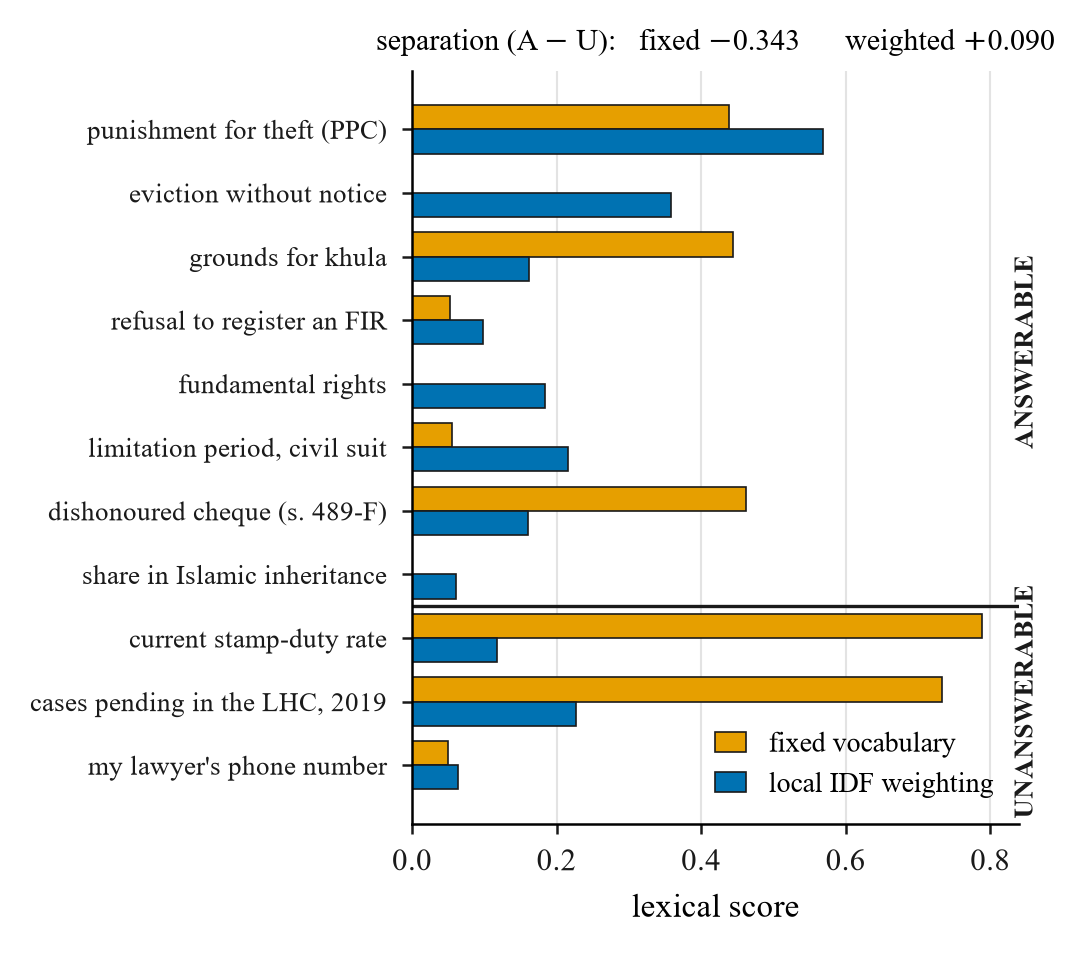
\includegraphics[width=\columnwidth]{figures/fig2_lexical.png}
\caption{The lexical signal on eleven diagnostic queries, under a fixed
stop-word vocabulary and under local IDF weighting~\eqref{eq:localidf}. The
fixed signal scores the unanswerable queries \emph{above} the answerable ones:
a question about a live stamp-duty rate repeats statutory vocabulary the corpus
does contain, and the signal rewards the repetition. Weighting by discriminating
power within the candidate pool reverses the ordering.}
\label{fig:lexical}
\end{figure}

The second signal was not a signal at all. The ensemble retriever exposes no
per-document scores, so every chunk was assigned a neutral $0.5$ embedding
similarity: $35\%$ of every confidence score was a fixed offset, contributed
identically to an exact statutory match and to an unanswerable question.
Recovering the ingestion-time passage vectors costs $26$\,ms for $19$ chunks
plus $150$\,ms for one query encoding, and yields a signal that does discriminate
--- though weakly. Averaged per query, answerable queries score $0.818$
(range $0.790$--$0.848$) against $0.789$ ($0.768$--$0.801$) for unanswerable
ones. The bands are narrow and adjacent, which is why the raw cosine must be
rescaled over the operating range rather than treated as a probability.

The third signal was unvalidated. The relevance grader runs on a small
fast-tier model, which was observed returning an array of $130$ grades for $8$
chunks; because the scorer pads and truncates its inputs, this was silently
accepted as a judgement that all eight chunks were irrelevant --- a malformed
response entering the audit trail indistinguishably from a considered one.
Length-checking the response and routing failures into the existing neutral
degradation path removes this. We note the general lesson: a signal whose
failure mode is a \emph{confident wrong value} rather than an absent value is
more dangerous than no signal, and only length validation distinguishes them.

\subsection{Repairing the Signals Does Not Separate Answerability}
\label{sec:answerability}
With the lexical signal corrected and the embedding signal supplied, the
aggregate score orders the two classes correctly --- mean $0.429$ for answerable
against $0.333$ for unanswerable --- but their \emph{ranges overlap}. Answerable
queries span $0.309$--$0.662$ and unanswerable ones $0.273$--$0.412$, so the
worst answerable query scores below the best unanswerable one. No threshold on
$c$ separates the classes; each cut only trades false refusals against false
answers.

This is the central negative result on abstention: the difference between these
classes is not one of degree in confidence, and treating it as one is a category
error. What distinguishes ``the current stamp-duty rate'' from ``the grounds for
\emph{khula}'' is not that the retrieved law is less similar --- it is that no
statute states a rate in force today. Deciding this from the query, before
evidence is weighed, is deterministic and costs nothing. On a set of $27$
queries constructed to stress the boundary, the query-side check admitted
$17/17$ answerable queries and identified $10/10$ unanswerable ones.

That set was written by the author while building the check, and both figures
must be read accordingly: constructing the boundary cases and the rule that
separates them together is a design activity, not an evaluation. The numbers
establish that the classes \emph{are} separable by a deterministic query-side
test --- the claim being made --- not that this rule generalises to queries it
was not written against. We state this here rather than in the Limitations
alone, since a precision figure quoted without its provenance invites exactly
the reading it does not support.

Precision matters more than recall here: a false positive refuses a question
the system could have answered, and the user cannot distinguish that from a
genuine gap in the law. Two false positives found during development are
instructive, both near-misses sharing surface vocabulary with an unanswerable
class --- ``how many \emph{days} do I have to file an appeal'' is a limitation
question, not a court statistic, and ``recover my lawyer's \emph{fee}'' is the
law of costs, not a personal record. Both are retained as regression tests.
Refusals name the reason and redirect to where the answer does live, since a
bare statement of failure is indistinguishable from a retrieval miss and merely
invites rephrasing.

One architectural defect accompanies this, reported for its failure mode rather
than as a contribution. Verified end-to-end after the fix, the stamp-duty query
still answered at $0.85$ confidence: a cache hit routes directly to the
finalising node, bypassing arbitration, so an answer produced by the defective
scorer outlived the correction of that scorer. The remedy was to version the
decision policy, so that changing it expires the answers it produced.

\subsection{The Harm Ratio and Its Sensitivity}
\label{sec:rho}
The decision rule of \eqref{eq:boundary} has one free parameter. Read in
reverse, it also tells us what an operating threshold set some other way
implicitly assumes, and that is worth doing before anything else. Our deployed
generation floor of $0.20$ was seeded as a percentile of a score distribution
and was never a statement about harm. It corresponds to $\rho = 4$: it commits
the system to a missed answer being \emph{four times worse} than a misstatement
of law, the inverse of the asymmetry the system is designed around. Nothing
connected the threshold to the harm it encodes until it was written down this
way.

Figure~\ref{fig:rho} sweeps $\rho$ over the measured confidences. The parameter
behaves as it should --- raising the penalty on wrong answers raises the
threshold and reduces coverage --- but the two curves move \emph{together}, and
no $\rho$ answers the answerable queries while refusing the unanswerable ones.
That is the overlap of Section~\ref{sec:answerability} seen through the decision
rule.

\begin{figure}[t]
\centering
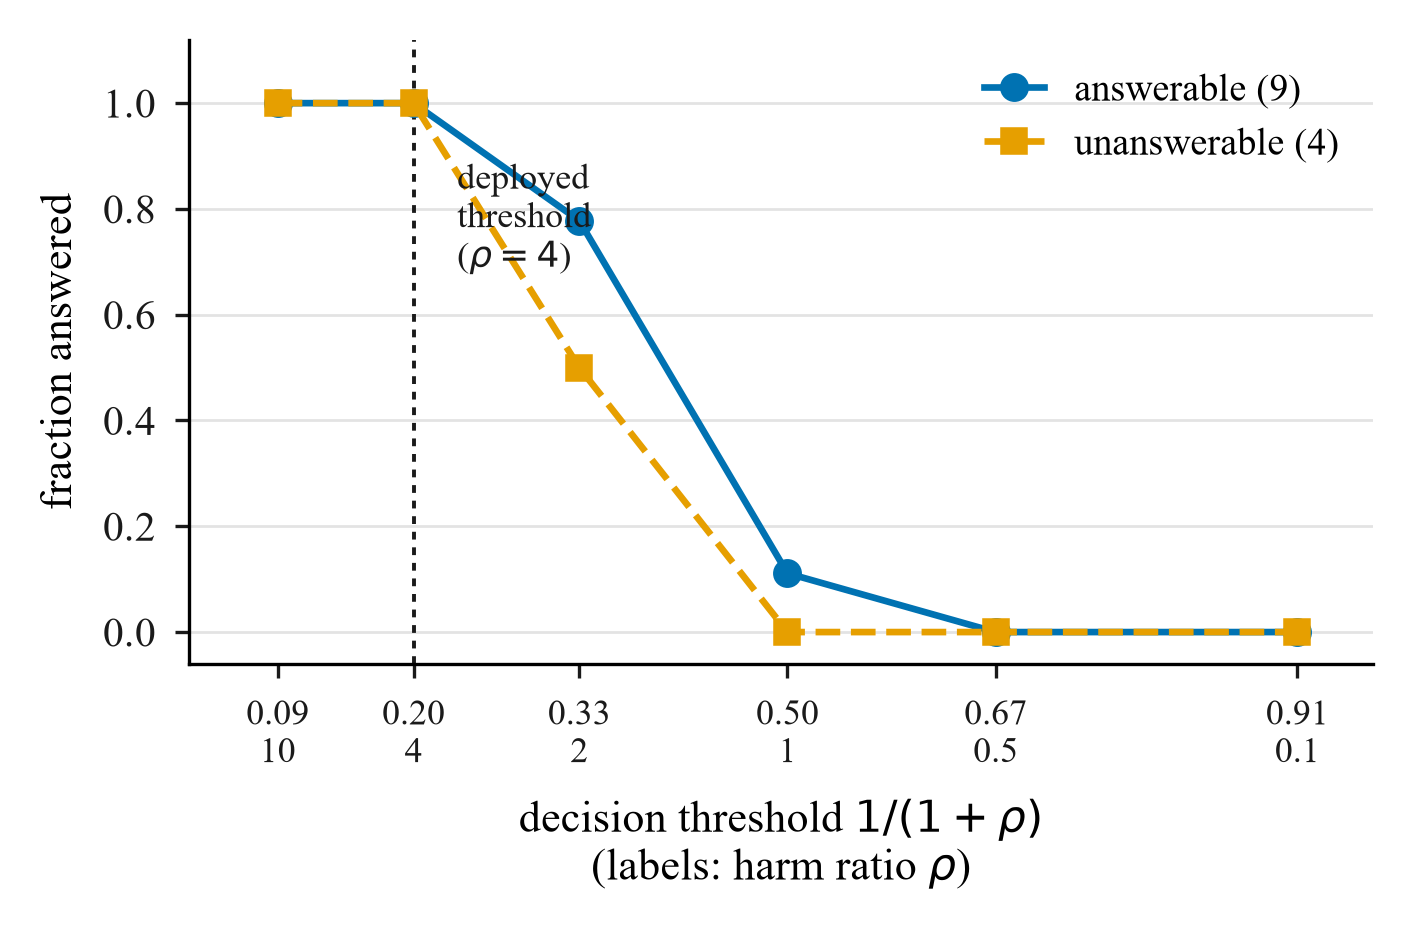
\includegraphics[width=\columnwidth]{figures/fig5_rho.png}
\caption{Coverage against the harm ratio, over the thirteen diagnostic queries.
The two curves move together across the whole sweep: no value of $\rho$ answers
the answerable questions while refusing the unanswerable ones. This is the same
overlap reported in Section~\ref{sec:answerability}, seen from the decision side
rather than the signal side.}
\label{fig:rho}
\end{figure}

Two practical consequences follow. First, $\rho$ governs only how conservative
the fallback is \emph{behind} the query-side check of
Section~\ref{sec:answerability}; it is not the mechanism that distinguishes
answerable from unanswerable, and presenting it as one would misattribute the
result. Second, plausible-looking harm assignments are more aggressive than
they appear. A utility matrix penalising a wrong answer at $-100$ against $+10$
for a correct one, $-10$ for an unnecessary refusal and $+5$ for a correct one
--- values that read as reasonable --- induces a threshold of $0.84$, above
every confidence we measured, and would refuse all traffic. We therefore retain
$\rho = 4$, which preserves the deployed operating point, and report the
assumption rather than presenting a tuned threshold as a principled one.

\subsection{Cross-Encoder Reranking: A Negative Result}
\label{sec:rerank}
Adding a cross-encoder reranker is the standard remedy for the symptom we faced
--- the correct statute retrieved but ranked below a lexically similar
competitor --- so we implemented and measured it rather than assuming it.
Table~\ref{tab:rerank} reports the decisive case. The query asks whether a
tenant may be evicted without notice in Punjab; the correct instrument is the
Punjab Rented Premises Act 2009, governing urban rental, and the competitor is
the Punjab Tenancy Act 1887, governing agricultural tenancy. Both are genuinely
about tenants and eviction, so this is an ambiguity of statutory scope rather
than a vocabulary gap, and it \emph{appeared} only as the corpus grew to include
provincial law.

\begin{table}[t]
\caption{Rank of the correct statute (Punjab Rented Premises Act 2009) and
median latency, at both retrieval depths. Lower rank is better; the top-ranked
statute after each stage is given, since what the reranker \emph{promotes} is
the diagnostic quantity.}
\label{tab:rerank}
\centering
\small
\begin{tabular}{@{}llcl@{}}
\toprule
Depth & Configuration & Rank & Top-1 statute \\
\midrule
$k{=}10$ & first stage           & 3  & Tenancy 1887 \\
(19)     & $+$ scope rules       & \textbf{1} & \textbf{Rented Premises 2009} \\
         & $+$ cross-encoder     & 10 & Tenancy 1887 \\
\midrule
$k{=}50$ & first stage           & 4  & Tenancy 1887 \\
(58)     & $+$ scope rules       & \textbf{1} & \textbf{Rented Premises 2009} \\
         & $+$ cross-encoder     & 24 & Tenancy 1887 \\
\bottomrule
\end{tabular}
\end{table}

The cross-encoder does not merely fail to help here; it moves the correct
statute \emph{away} from the top, from rank 3 to rank 10 at the deployed depth
and from 4 to 24 when the pool is widened, and at both depths it promotes the
agricultural statute --- precisely the confusion it was introduced to resolve.
The degradation grows with pool size, which is the signature of a scoring
function that is not merely noisy but systematically ordered against the target:
more candidates give it more opportunities to prefer the wrong one. The
deterministic scope rules place the correct statute first at both depths in
under a millisecond, against $0.73$\,s and $2.43$\,s for the reranker.

The failure is not uniform, and reporting it as such would overstate it. Across
six queries the reranker improved three (the \emph{khula} target from rank 8 to
4, an FIR-registration query from 2 to 1, a theft query from 3 to 1), left two
unchanged, and badly worsened one. But the one it worsens is the case that
motivated it. The queries it improves were already nearly correct --- the right
statute was in the top three --- so it is sharpening rankings that did not need
sharpening while inverting the one that did.

We attribute this to a train/test distribution shift rather than to model
capacity. The checkpoint is trained on MS MARCO, whose relevance judgements
concern short web passages answering informational queries. The distinction the
query turns on --- whether \emph{tenant} means a cultivator under an 1887
revenue statute or an occupant of urban premises under a 2009 one --- is a
matter of legislative scope, and both statutes discuss tenants, eviction and
notice. A relevance model trained on topical overlap has no representation of
which instrument \emph{governs}. Prior work reports the same direction of
effect, attributing degraded legal case retrieval to domain mismatch on long
legal text unlike the reranker's training data~\cite{hou2024clerc}; that this
reproduces on statutory retrieval in a different jurisdiction and language
setting suggests a property of the domain rather than of one corpus.

Widening first-stage retrieval from $10$ to $50$ candidates was reverted
alongside it: without an effective reranker, additional depth is additional
noise. Under the wider pool the \emph{khula} query's target fell from rank 8 to
14, and Table~\ref{tab:rerank} shows the reranker's own error growing with the
pool it is given.

We report this as a negative result rather than omitting it. A legal-domain
cross-encoder, or one fine-tuned on the labelled set once it exists, may well
succeed where the generic model failed; the finding is that the off-the-shelf
model is actively harmful on this text, not that reranking is unsound.

\subsection{Domain Fine-Tuning: Large In-Distribution Gains That Do Not Transfer}
\label{sec:finetune}
The diagnosis of Section~\ref{sec:rerank} left a specific gap. On $200$ held-out
constitutional questions the correct article is retrievable at dense depth $50$
for $89\%$ of them but reaches rank~1 for only $43.5\%$ --- a $45$-point
\emph{ranking} deficit rather than a recall one. Reranking having failed, the
remaining hypothesis was that a general-purpose multilingual embedding model
does not know Pakistani statutory language. We tested it by fine-tuning.

Two models were trained, deliberately at different scales and from different
sources, so that any pattern could be checked for consistency rather than read
off a single run:

\begin{itemize}
\item \textbf{Constitutional}: 471 question/article pairs from LEGAL-UQA.
\item \textbf{General}: 4{,}692 pairs spanning constitutional, criminal,
evidence, civil procedure and family law, built from a citation-annotated corpus
and verified as described in Section~\ref{sec:citationdata}. A third of its
queries are in Urdu script.
\end{itemize}

Both use \texttt{multilingual-e5-base} with multiple-negatives ranking loss and
hard negatives mined from the deployed retriever, and both are split by connected
components over shared gold chunks so that no gold chunk appears in both halves.
Table~\ref{tab:setup} gives the configuration in full, so that the comparison
can be reproduced or contradicted.

\begin{table}[t]
\caption{Fine-tuning configuration. Identical apart from the training corpus,
so the difference between the two models is the data and not the recipe.}
\label{tab:setup}
\centering
\small
\begin{tabular}{@{}lcc@{}}
\toprule
Property & constitutional & general \\
\midrule
Training pairs        & 471 & 4{,}692 \\
Held-out pairs        & 121 & 1{,}191 \\
Legal domains         & 1 & 5 \\
Urdu-script queries   & 0\% & 32\% \\
Source                & LEGAL-UQA & citation corpus \\
\midrule
Base model            & \multicolumn{2}{c}{\texttt{multilingual-e5-base}} \\
Loss                  & \multicolumn{2}{c}{multiple-negatives ranking} \\
Hard negatives        & \multicolumn{2}{c}{mined from the deployed retriever} \\
Epochs / batch / lr   & \multicolumn{2}{c}{2 / 12 / $2\times10^{-5}$} \\
Max sequence length   & \multicolumn{2}{c}{224 tokens} \\
Train/test split      & \multicolumn{2}{c}{connected components over $G_q$} \\
Significance test     & \multicolumn{2}{c}{McNemar, paired on $Q$} \\
\bottomrule
\end{tabular}
\end{table}

\begin{figure}[t]
\centering
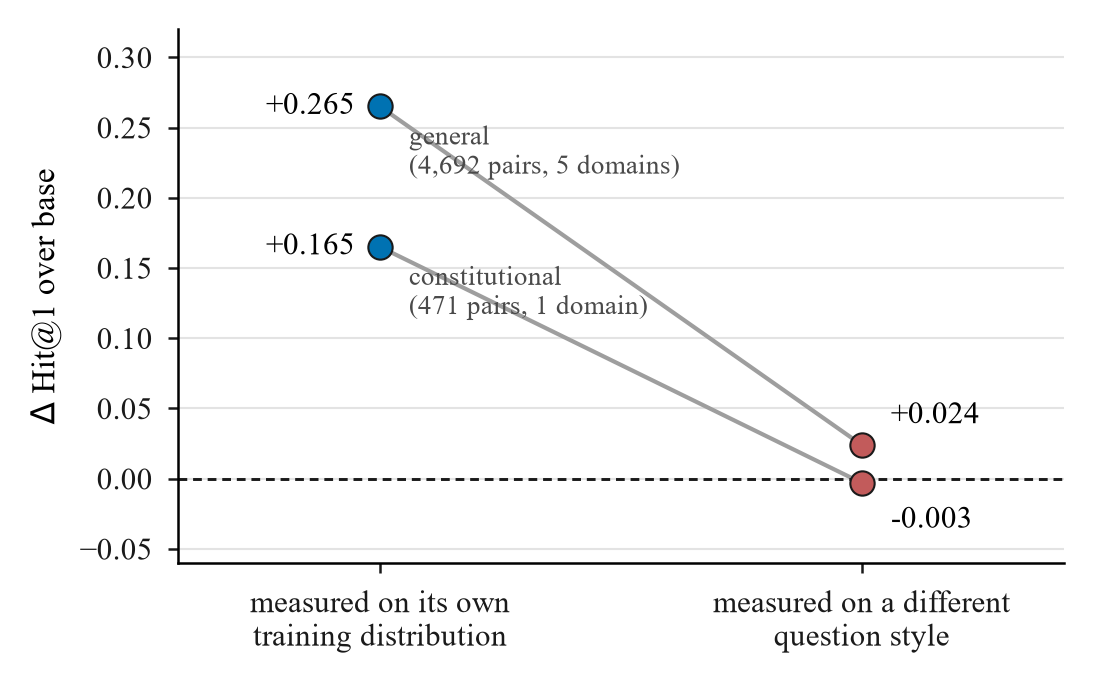
\includegraphics[width=\columnwidth]{figures/fig4_transfer_collapse.png}
\caption{The transfer result. Two models trained independently, on different
sources, at a tenfold difference in scale, lose almost the whole of their gain
when the question style changes. The left-hand points are what an
in-distribution evaluation would report; the right-hand points are what a
deployment would experience. The constitutional model's apparent $0.766$ on its
own distribution is excluded as memorisation and is not plotted
(Section~\ref{sec:leakage}).}
\label{fig:collapse}
\end{figure}

\begin{table}[t]
\caption{Hit@1 for each model, evaluated on questions drawn from its OWN
training distribution and from the other. Each model's out-of-distribution
column is the honest measure of transfer.}
\label{tab:finetune}
\centering
\small
\begin{tabular}{@{}lccc@{}}
\toprule
Test set & base & constitutional & general \\
\midrule
Citation-style, held out & 0.4148 & \emph{0.4114} & \textbf{0.6801} \\
(general's distribution)  &        & $-0.3$ & $+26.5$ \\
\midrule
LEGAL-UQA style, held out & 0.5234 & \textbf{0.7656}$^\dagger$ & \emph{0.5469} \\
(constitutional's dist.)  &        & --- & $+2.4$ \\
\bottomrule
\end{tabular}

\vspace{2pt}
\footnotesize Italics mark the out-of-distribution measurement for each model.
$^\dagger$Not reportable: $106$ of these $128$ questions, and $48$ of $59$ gold
chunks, were in the constitutional model's training set (Section~\ref{sec:leakage}).
\end{table}

Table~\ref{tab:finetune} reports Hit@1 for every model on both test sets, and
Figure~\ref{fig:collapse} states the same result as transfer. Measured on its
own distribution the
general model gains $+26.5$ Hit@1, a $64\%$ relative improvement, significant at
$p\approx0.0005$ by McNemar's test on $531$ improved against $123$ worsened
pairs. Measured on questions written by a different generator, the same model
gains \textbf{$+2.4$}, with $31$ improved against $22$ worsened --- close to a
coin flip.

The constitutional model shows the same pattern from the other direction. On
its own distribution it gains $+16.5$ dense and $+6.6$ once fused with BM25
(Section~\ref{sec:hybrid}); on citation-style questions it gains
\textbf{$-0.3$}. We verified that this second figure is clean: none of the
$1{,}191$ citation-style test questions appear in its training set.

Ten times the training data, five legal domains and two scripts bought a larger
in-distribution number and essentially nothing out of it. The effect replicates
across two models trained independently on different sources at different
scales, which is what makes it a finding about the method rather than about one
run.

\subsection{Why the Fusion Layer Absorbs the Gain}
\label{sec:hybrid}
A second reduction occurs before deployment. The figures above are dense-only;
the deployed retriever fuses BM25 at $0.6$ with dense at $0.4$. Rebuilding both
indexes at identical sequence length so that only the weights differ, the
constitutional model's $+16.5$ becomes $\mathbf{+6.6}$ under fusion.

The mechanism is visible in the baselines: hybrid base scores $0.5207$ against
dense base $0.4380$, so BM25 was already supplying $+8.3$ points on its own.
Much of what fine-tuning teaches the dense channel, the lexical channel already
knew, and overlapping gains do not add.

Fusion also \emph{repairs} the characteristic damage. Under dense-only retrieval
four queries fell from a found rank to absent, all of them exact-citation
lookups; under fusion the worst regression is rank~1 to rank~3. A system
reporting only its dense ablation would overstate both the benefit and the harm.

\subsection{Failures Resolved Without Additional Data}
Three queries that failed before the corpus expansion were re-tested after it.
All three now succeed, and none was fixed by the additional data. A maintenance
query in Roman Urdu failed because a model-assigned language label overrode the
script actually observed; the eviction query failed on the statutory-scope
ambiguity of Section~\ref{sec:rerank}; and the \emph{khula} query failed because
the classifier's case-type verdict was computed and then discarded one node
later, so the turn was routed to clarification and never retrieved anything.
Each was a defect in the handling of a signal, not an absence of law, and we
note that a purely data-centric response --- ingesting more statutes --- would
have resolved none of them while appearing to be the obvious remedy.

\subsection{Three Contaminations, Each Found by Looking}
\label{sec:leakage}
Every fine-tuning result above survived a contamination check that removed an
earlier, better-looking number. We report the three failures because each was
invisible in the metrics and each would have inflated a headline figure.

\emph{The index contained the test answers.} The constitutional collection held
$619$ generated question/answer pairs alongside $305$ article extracts, all
tagged as the Constitution, and the generated pairs contained each evaluation
question verbatim. They accounted for $81$--$100\%$ of retrieved chunks on
ordinary constitutional queries. Evaluating before removing them would have
retrieved each question's own answer at rank~1.

\emph{The gold labels were systematically wrong.} Joining evaluation questions
to gold passages by section heading produced an off-by-one: the source PDF's
marginal notes are extracted as heading-only stubs, so the heading of Article~25
matched a stub rather than the chunk holding its text. Retrieval was returning
the correct chunk and the evaluation scored it as a miss. The signature was
Hit@1 of exactly $0.000$ across $568$ questions --- a number implausible enough
to prompt a check. Rebuilding the join on verbatim body $n$-grams moved MRR from
$0.114$ to $0.581$ with no change to the system.

\emph{The test set shared targets with training.} For the cross-style
evaluation, $99$ of $121$ candidate questions had gold chunks that were also
training positives for the general model --- different questions, identical
targets. This is target leakage rather than question leakage, and it is not
caught by deduplicating queries. Filtering to genuinely unseen targets across
the full $592$-question set left $128$ usable questions.

A fourth check applies to Table~\ref{tab:finetune}. The constitutional model's
apparent $0.7656$ on LEGAL-UQA-style questions is memorisation: $106$ of those
$128$ questions were in its training set, because that set is drawn from
LEGAL-UQA. Between them the two models had consumed $464$ and $471$ of the $592$
available questions, leaving only $22$ unseen by both --- too few to support a
three-way comparison. The out-of-distribution columns are the only ones we
report.

\subsection{What Is Not Yet Measured}
\label{sec:notmeasured}
The ranking and selective-prediction metrics of Section~\ref{sec:eval} ---
Hit@$k$, MRR, nDCG@$k$, risk--coverage curves and expected calibration error ---
require the pooled labelled set, which is not yet of sufficient volume to report.
We state this rather than substitute proxies. The same set would settle the
generalisation question left open in Section~\ref{sec:answerability}: the
query-side check needs to be run against queries authored independently of it,
with the unanswerable classes labelled by someone who did not write the rules,
before its precision can be claimed as a property of the method rather than of
the examples it was built from. In particular the calibration
transforms of Section~\ref{sec:calib} remain identity maps: the architecture
places Platt scaling and isotonic regression on the correct path and the fitted
parameters are the only missing component, so the confidence values reported
above are \emph{ranked} scores and are not claimed to be calibrated
probabilities. This is why the contribution is stated as selective prediction
rather than calibrated prediction.

\section{Discussion and Limitations}
\label{sec:disc}

\subsection{Why Fine-Tuning Did Not Generalise}
\label{sec:whynot}
Sorting every retrieval intervention we measured by whether its effect
survived a change of question style produces a clean split:

\begin{center}
\small
\begin{tabular}{@{}lc@{}}
\toprule
Transferred & Did not \\
\midrule
statute-scope rules (rank $12\!\to\!1$) & fine-tuned embeddings ($+2.4$) \\
query-side answerability check & cross-encoder rerank (rank $3\!\to\!10$) \\
corpus repairs & fusion-weight tuning (no gain) \\
\bottomrule
\end{tabular}
\end{center}

The dividing line is not complexity or cost but \emph{what the intervention
encodes}. Everything on the left encodes a property of the law or the documents;
everything on the right learns a mapping from question surface form to passage.
Legal language is why this matters more here than elsewhere: a statutory corpus
is small, highly structured, and written in a register no user employs, so the
gap between a question and its answer is one of \emph{register}, not of topic. A
model fitted to one generator's phrasing closes that specific gap and a
differently-phrased question reopens it, whereas the rule that the Punjab Rented
Premises Act 2009 governs shops and houses while the Punjab Tenancy Act 1887
governs cultivators holds however the question is worded --- and cost four
milliseconds.

The errors agree with the aggregates. One exact-citation lookup ---
``What was omitted by S.R.O. No. 1278~(1)~85?'' --- fell from rank~1 to absent
under the cross-encoder, under the constitutional model \emph{and} under the
general model: all three traded lexical precision for semantic similarity,
which is what optimising a dense objective on paraphrased questions rewards.
That BM25 fusion partially repairs the damage says what was lost was lexical
rather than legal.

We do not claim fine-tuning cannot work for legal retrieval, only that training
on one generator's questions produces a model fitted to that generator, that
this is invisible when the test set shares the generator, and that the
in-distribution number is therefore not evidence of deployment benefit. A model
trained on diverse human-authored queries might behave differently; no such set
exists for this jurisdiction, so we could not test it.

\subsection{Leakage-Free Evaluation Is the Load-Bearing Component}
\label{sec:whyleakage}
Three of our results were wrong before they were checked, and each time the
flattering version was the wrong one (Section~\ref{sec:leakage}). We draw three
practical conclusions.

\emph{Contamination in retrieval systems has more surfaces than in
classification.} A question can leak, a gold label can leak, and --- as here ---
the \emph{index} can leak, because the corpus under evaluation is itself a
system component. Deduplicating queries catches none of the latter two.

\emph{Generated evaluation sets carry their generator's signature.} Both
datasets that supplied our labels were LLM-generated against statute. That makes
them usable as training signal, since the citation is a checkable label, and
unreliable as benchmarks, since a model trained on one generator is tested on its
own idiom. The $+26.5$ to $+2.4$ collapse is the size of that effect.

\emph{The measurement protocol determined the conclusions more than any
technique did.} Our largest reported gain, $+6.6$ Hit@1 under fusion, is the one
that survived every check. The three larger numbers did not survive. A system
paper that reports only its best configuration on its own evaluation set is not
making a weaker claim than ours --- it is making an unfalsifiable one.

\subsection{Future Work}
\label{sec:future}
The immediate constraint is not method but measurement. Every evaluation asset
used here is either authored by the system's developer or drawn from a training
generator, and the honest consequence is that we cannot presently prove an
end-to-end improvement.

\emph{An independent benchmark, frozen before use.} We have identified $3{,}852$
Pakistani legal questions used to train none of our models. Labelling a subset
with two annotators, reporting Krippendorff's $\alpha$, and \emph{freezing} half
before any development begins would give the first evaluation set this work
could not have tuned against. Pre-registering the predicted effect and opening
the frozen half once is what would convert a measurement into evidence.

\emph{Structure-aware chunking.} Our strongest untested lever follows the
principle of Section~\ref{sec:whynot}: it is structural. Between $20$ and $27\%$
of each collection is under $200$ characters --- heading fragments competing for
retrieval slots --- and $11\%$ of failures are recall rather than ranking.
Aligning chunk boundaries to statutory structure and prepending instrument and
section metadata before embedding addresses both, and should place the citation
string inside the passage where the lexical channel can reach
it~\cite{metadatarag2026,reliablelegalrag2025}.

\emph{Generation correctness.} Every number in this paper measures retrieval.
Users receive generated answers, and we verify that answers are \emph{grounded}
in retrieved text without verifying that they are \emph{correct}. Those differ,
and the difference is where a legal assistant causes harm: a fluent answer,
correctly grounded in a correctly retrieved provision, that misstates what the
provision means. Even at perfect retrieval we would have no evidence of legal
correctness. Establishing that requires practitioner adjudication of emitted
answers, and it is the measurement we would prioritise above all others.

\emph{Fitting the calibration layer.} The conformal and harm-matrix machinery of
Sections~\ref{sec:calib} and~\ref{sec:abstain} is implemented and inert pending
labelled data. Once fitted, the coverage guarantee becomes reportable and the
harm ratio can be elicited from practitioners rather than inherited from a
threshold.

\subsection{Observations on the Governance Layer}
Four further observations generalise beyond this system, and each concerns the
governance layer rather than any model in it.

\emph{A policy is only as good as the paths that consult it.} An
intent-classification shortcut answered certain turns without entering the graph,
bypassing the injection gatekeeper; a result cache produced the same failure at
the opposite end, serving stored answers without consulting the arbitration that
would have refused them, so a correction to the decision logic silently did not
apply. Neither component was weak; neither was reached. Any robustness or
refusal rate measured in that configuration is computed only over traffic that
arrived at the defended component --- a measurement error, not a model error.
The remedies were structural: one enforced output path, and versioning the
decision policy so cached answers cannot outlive the logic that produced them.

\emph{Keyword safety filters collide with domain vocabulary.} Our injection
filter matched a power-of-attorney question containing ``unrestricted agent''.
A false positive here refuses a user with a genuine legal problem, which argues
for narrow patterns backed by a model layer --- applied where a model consumes
untrusted text, rather than uniformly.

\emph{A confidence signal can be inverted, not merely weak, and the aggregate
will hide it.} The composite of Section~\ref{sec:signaldiag} behaved plausibly
while one component was anti-correlated with correctness and two others were
constant. We would encourage reporting per-signal separation, not only aggregate
confidence, wherever heterogeneous evidence is combined.

\emph{Formalising an informal rule changes behaviour, and not only where
expected.} Replacing the threshold ladder with \eqref{eq:losses} left the
answer/refuse boundary at the same $0.20$ by derivation, but changed when the
system asks a clarifying question: asking must now earn its friction against the
disagreement it could resolve, so weak but internally consistent evidence is
refused rather than queried. We regard this as correct --- a clarification
cannot improve an estimate the signals already agree on --- but it was not
anticipated when the derivation was undertaken.

The work has substantive limitations, which we state rather than leave to be
discovered. \emph{Calibration is not fitted.} The Platt and isotonic transforms
of Section~\ref{sec:calib} are implemented and remain identity maps pending
labelled data, so every confidence value we report is a ranked score and not a
probability; the split-conformal layer~\cite{angelopoulos2021conformal} that
would supply a coverage guarantee is likewise implemented and unfitted. This is
the single largest gap between the architecture and the evidence for it.
\emph{Relevance judgements are the authors' own}, not adjudicated by qualified
practitioners, which is a real constraint on any claim about legal correctness
as opposed to retrieval quality. \emph{Evaluation queries were authored
alongside the system}, making them a bootstrap rather than an independent
benchmark. \emph{The harm ratio $\rho$ is not elicited}, but set to the value implied by
the deployed threshold, so \eqref{eq:boundary} makes the assumption auditable
without making it correct; eliciting it is the obvious next step, and
\eqref{eq:boundary} is what makes that a well-posed question. \emph{Coverage is single-jurisdiction},
and the corpus is weighted towards statute relative to case law, so performance
on precedent-driven questions is likely weaker than on statutory ones. Finally,
the pooled relevance judgements bound the depth at which ranking metrics are
meaningful, and we report only cut-offs within that depth.

\section{Conclusion}
Legal question answering in a low-resource, code-switched jurisdiction is
neither served by transplanting an English common-law pipeline nor adequately
measured by answer quality alone. We described a governance architecture that
admits deterministic statutory computation as evidence its own verifier accepts,
routes every query through an explicit decision between answering, clarifying
and refusing, and records for each turn the evidence behind what it emitted.

Our measurements argue that the hard part of abstention here is not estimating
confidence better but recognising that confidence is the wrong quantity. The
highest-weighted component of our own confidence score was anti-correlated with
answerability, favouring unanswerable questions by $0.343$; repairing it
restored the ordering yet left the two classes overlapping, and separation was
obtained only by asking, before any evidence was weighed, whether the corpus
could hold the answer at all. That question is answerable deterministically, and
in a domain where a confident wrong answer causes material harm, we would rather
decide it that way than infer it from a score.

A second theme runs through the results and, we think, generalises further. The
interventions that improved this system durably were those encoding something
true about the law or the documents --- which instrument governs a dispute, what
kind of fact a statute can state, what the corpus actually contains. The
interventions that learned a mapping from question phrasing to passage produced
larger headline numbers and did not survive a change of question style. That
distinction was only visible because three of our own results were wrong before
they were checked, and the flattering version was the wrong one every time.

We therefore close on the measurement rather than the method. Every evaluation
asset used here is authored by the system's developer or drawn from a training
generator, and the honest consequence is that we cannot yet prove an end-to-end
improvement in the thing users actually receive: a generated statement of law.
Establishing that requires an independent benchmark frozen before development
and practitioner adjudication of emitted answers. For a system whose purpose is
to tell people what the law says, that is not an extension of the work. It is
the work.

\section*{Ethical Considerations}
The system provides legal information, not legal advice, and every answer
carries an explicit disclaimer directing users to a qualified practitioner.
Refusal is treated as a first-class outcome precisely because a confident wrong
answer in this domain can cause material harm. Stored records mask personally
identifying information, and audit records are retrievable only by the user who
produced them.

%-----------------------------------------------------------------------------
\section*{Acknowledgment}
\TODO{supervisor, department, any funding}

\bibliographystyle{IEEEtran}
\bibliography{references}

\end{document}
